\documentclass{beamer}

\mode<presentation>{%
  \usetheme[block=fill,progressbar=frametitle]{metropolis}
  \setsansfont[BoldFont={Fira Sans SemiBold}]{Fira Sans Book}
}
\setbeamercolor{background canvas}{bg=white}

\usepackage{appendixnumberbeamer}
\usepackage[font=tiny]{caption}
\usepackage{graphicx}
\usepackage{pifont}
% \usepackage{booktabs}

\newcommand{\norm}[1]{\left\lVert#1\right\rVert}


\title{Biclustering with heterogeneous variance}
\author{Guanhua Chen, Patrick F. Sullivan, and Michael R. Kosorok}
\date{July 23, 2013}

\begin{document}

\begin{frame}
\titlepage%
\end{frame}

\begin{frame}{Problem}
  How to \textbf{cluster} data using \textbf{relevant factors} while
  \textbf{excluding irrelevant information and noise.}
  \begin{figure}
    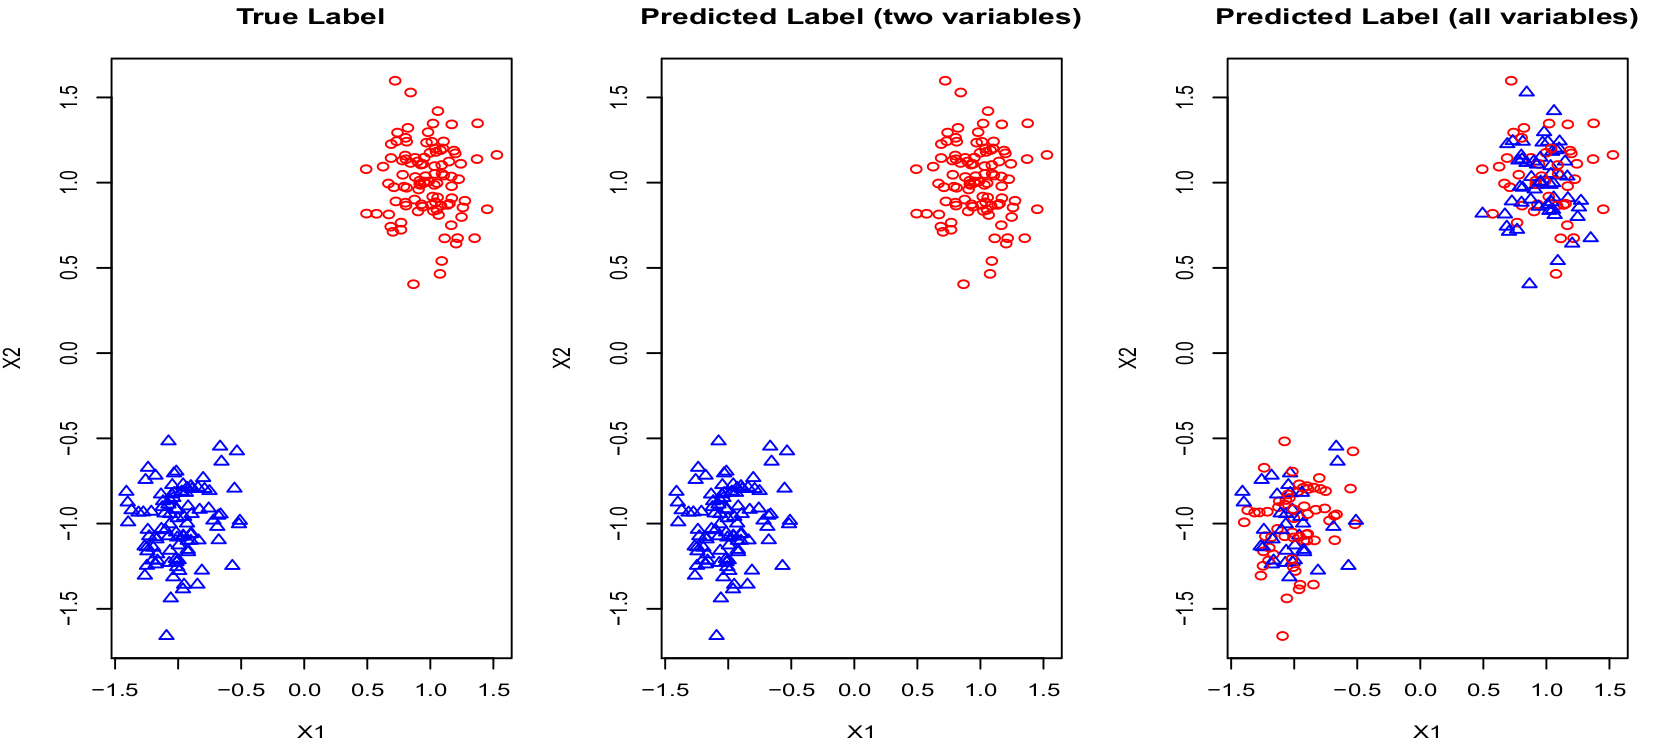
\includegraphics[width=\linewidth]{figures/fig1v2.png}
    \caption{Data set contains two clusters determined by two variables $X_1$
      and $X_2$ such that points around $(1,1)$ and $(-1,-1)$ naturally form
      clusters. There are 200 observations (100 for each cluster) and 1,002
      variables ($X_1$, $X_2$ and 1,000 random noise variables). We plot the
      data in the 2D space of $X_1$ and $X_2$. Graphs with true cluster labels
      and predicted cluster labels obtained by clustering using only $X_1$ and
      $X_2$ and clustering by using all variables are laid from left to right.
      The predicted labels are the same as the true labels only when $X_1$ and
      $X_2$ are used for clustering; however, the performance is much worse
      when all variables are used.}
  \end{figure}
\end{frame}

\section{Background}

\begin{frame}{Biclustering}
  \begin{enumerate}
    \item Rather than cluster features in sample-space or samples in feature
      space, cluster both simultaneously.
    \item Clusters correspond to some sort of functional relationship between
      rows and columns, e.g.:
      \begin{itemize}
        \item Minimum variance across rows/columns/values
        \item Constant rows/columns
      \end{itemize}
  \end{enumerate}
\end{frame}

\begin{frame}{Biclustering Example I (BicAT Yeast)}
  \begin{figure}
    % \includegraphics[width=\linewidth]{figures/heatmap.png}
    \includegraphics[width=\linewidth,height=\textheight,keepaspectratio]{figures/heatmap.png}
    \caption{Heatmap of yeast microarray data from BicAT dataset.}
  \end{figure}
\end{frame}

\begin{frame}{Biclustering Example II (BicAT Yeast)}
  \begin{figure}
    % \includegraphics[width=\linewidth]{figures/heatmapBC.png}
    \includegraphics[width=\linewidth,height=\textheight,keepaspectratio]{figures/heatmapBC.png}
    \caption{Biclustered heatmap of yeast microarray data from BicAT dataset.}
  \end{figure}
\end{frame}

\begin{frame}{Sparsity + biclustering = \ding{170}}
  \begin{enumerate}
    \item Finding optimal set of biclusters is NP-Complete.
      \begin{itemize}
        \item Computationally expensive
      \end{itemize}
    \item Algorithms are unsupervised.
      \begin{itemize}
        \item Difficult to tell if solution is optimal
        \item Often resort to different clustering methods and majority voting
          (even more expensive!)
      \end{itemize}
    \item \textbf{Nifty trick:} for sparse matrices, SVD can compute biclusters
      without the need for matrix permutations.
  \end{enumerate}
\end{frame}

\begin{frame}{Sparsity}
  \begin{enumerate}
    \item Genotype data is very high-dimensional in terms of features.
    \begin{itemize}
      \item Only a subset of features may contribute to a trait.
    \end{itemize}
    \item A matrix is sparse if over half its elements are 0.
    \item Raw data will be a combination of sparse signal ($\Xi$) and iid noise
      ($\Phi$).
  \end{enumerate}
  \begin{align*}
    \textbf{X} &= \textbf{\Xi} + \textbf{\Phi}
  \end{align*}
\end{frame}

\begin{frame}{Sparse SVD (SSVD) Trick}
  \begin{enumerate}
    \item SSVD computes sparse singular vectors.
    \item Submatrices formed by singular vector outer products.
      \begin{itemize}
        \item Outer products correspond to biclusters.
      \end{itemize}
    \begin{align*}
      \textbf{X} &\approx \textbf{U}\textbf{S}\textbf{V}^T = \sum_{i=1}^r s_i \textbf{u}_i\textbf{v}_i^T\textrm{, where }
    \end{align*}
    \begin{align*}
      \textbf{X} &\in \mathbb{R}^{n \times p}\textrm{, } \textbf{U} \in \mathbb{R}^{n \times r}\textrm{, } \textbf{V} \in \mathbb{R}^{r \times p}\textrm{, } \\
      &\textbf{S} \in \mathbb{R}^{r \times r}\textrm{, and } r \ll \textrm{rank}(\textbf{X})
    \end{align*}
  \end{enumerate}
\end{frame}

\begin{frame}{SSVD (I)}
  \begin{enumerate}
    \item SSVD singular vectors are not \textit{exactly} singular vectors.
    \item Method imposes an adaptive $L_1$ penalty on singular vectors to
      enforce sparsity.
    \item These vectors are termed \textbf{SSVD layers}.
  \end{enumerate}
\end{frame}

\begin{frame}{SSVD (II)}
  \begin{align*}
    \textrm{Minimize: }&\norm{\textbf{X} - s\textbf{u}\textbf{v}^T}_F^2 + \lambda_u P_1(s\textbf{u}) + \lambda_v P_2(s\textbf{v})\textrm{, where } \\
    \\
    &P_1(s\textbf{u}) = P_1(\tilde{\textbf{u}}) = \sum_{i=1}^n w_{1,i} |u_i|\textrm{, } \\
    &P_2(s\textbf{v}) = P_2(\tilde{\textbf{v}}) = \sum_{j=1}^d w_{2,i} |v_i|\textrm{, } \\
    &\textbf{w}_1 = |\tilde{\textbf{u}}|^{-\gamma_1}\textrm{, and } \\
    &\textbf{w}_2 = |\tilde{\textbf{v}}|^{-\gamma_2}
  \end{align*}
\end{frame}

\section{HSSVD Model}

\begin{frame}{The HSSVD Model (I)}
  \begin{block}{HSSVD}
    Heterogeneous sparse singular value decomposition
  \end{block}
  \begin{enumerate}
    \item SSVD and other methods cluster around means.
    \item Hypothesis: Cancer genetic and epigenetic patterns can be
      characterized by means \textbf{and} variance.
    \item Method: HSSVD modifies the SSVD algorithm to use both for computing
      biclusters.
  \end{enumerate}
  \begin{align*}
    \textbf{X} &= \textbf{\Xi} + \rho^2 \textbf{\Sigma} \times \textbf{\Phi} + b\textbf{J}
  \end{align*}
\end{frame}

\begin{frame}{The HSSVD Model (II)}
  \begin{align*}
    \textbf{X} = & \textbf{\Xi} + \rho^2 \textbf{\Sigma} \times \textbf{\Phi} + b\textbf{J} \\
    \\
    \textbf{X} &\rightarrow \textrm{raw data} \\
    \textbf{\Xi} &\rightarrow \textrm{signal means} \\
    \textbf{\Sigma} &\rightarrow \textrm{signal variances} \\
    \textbf{\Phi} &\rightarrow \textrm{noise} \\
    \textbf{J} &\rightarrow \textrm{matrix of 1's} \\
    \rho, b &\rightarrow \textrm{constants}
  \end{align*}
\end{frame}

\begin{frame}{The HSSVD Algorithm (I)}
  \begin{enumerate}
    \item Standardize raw input $\textbf{X}_{origin}$ with overall mean
      $\hat\mu$ and std dev $\hat\sigma$. ($\textbf{X} = (\textbf{X}_{origin}-\hat\mu \textbf{J})/\hat\sigma$)
    \item Quadratic rescaling: Apply SSVD on $\textbf{X}^2 - \textbf{J}$ to
      obtain the approximation matrix $\textbf{U}$.
    \item Mean search:
      \begin{itemize}
        \item Let $\textbf{Y} = \textbf{X}/\sqrt{\textbf{U} + \textbf{J} -
          c\textbf{J}}$.
        \item Apply SSVD on $\textbf{Y}$ to obtain $\tilde{\textbf{Y}}$.
      \end{itemize}
  \end{enumerate}
\end{frame}

\begin{frame}{The HSSVD Algorithm (II)}
  \begin{enumerate}
    \setcounter{enumi}{3}
    \item Variance search:
    \begin{itemize}
      \item Compute $\textbf{Z}_{origin} = \log{(\textbf{X} -
        \tilde{\textbf{Y}}\times \sqrt{\textbf{U} + \textbf{J} - c\textbf{J}})}^2$.
      \item Then, center $\textbf{Z}_{origin}$ to obtain $\textbf{Z}$. 
      \item Perform SSVD on $\textbf{Z}$ to obtain $\tilde{\textbf{Z}}$.
    \end{itemize}
    \item Background estimation: 
      \begin{itemize}
        \item Compute $\textbf{P}$, an $n \times p$ matrix of indicators for
          whether an entry belongs to the background cluster.  ($P_{ij} = 1$ if
          $\tilde{Y}_{ij}$ and $\tilde{Z}_{ij}$ are $0$.) 
        \item Then, estimate $\hat{b} = \frac{\textbf{1}^T (\textbf{X}_{origin}
          \times \textbf{P}) \textbf{1}}{\textbf{1}^T \textbf{P} \textbf{1}}$.
        \item Then, estimate $\hat{\rho} = \frac{\textbf{1}^T (\textbf{X}_{origin}
          \times \textbf{P} - \hat{b}\textbf{P})^2 \textbf{1}}{\textbf{1}^T \textbf{P} \textbf{1} - 1}$.
      \end{itemize}
  \end{enumerate}
\end{frame}

\begin{frame}{The HSSVD Algorithm (III)}
  \begin{enumerate}
    \setcounter{enumi}{5}
    \item Scale back:
    \begin{itemize}
      \item Define $\textbf{P}_1 = \{p_{ij}\}$, with $p_{ij}=1$ if $\tilde{\textbf{Y}}_{ij} = 0$, and $p_{ij}=0$ otherwise.
      \item Define $\textbf{P}_2 = \{p_{ij}\}$, with $p_{ij}=1$ if $\tilde{\textbf{Z}}_{ij} = 0$, and $p_{ij}=0$ otherwise.
      \item Compute mean approximation $(\textbf{\Xi} + b\textbf{J})$ from
        $\hat{\sigma} (\tilde{\textbf{Y}} \times \sqrt{\textbf{U} + \textbf{J}
        - c\textbf{J}}) + \hat{\mu}(\textbf{J} - \textbf{P}_1) +
        \hat{b}\textbf{P}_1$.
      \item Compute variance approximation $(\rho\textbf{\Phi})$ from
        $\big(\hat{\rho}^2 \textbf{P}_2 + \hat{\sigma}^2 (\textbf{J} -
        \textbf{P}_2)\big) \times \exp{\tilde{\textbf{Z}}}$.
    \end{itemize}
  \end{enumerate}
\end{frame}

\section{Results}

\begin{frame}{Hypervariation of Methylation in Cancer (I)}
  \begin{figure}
    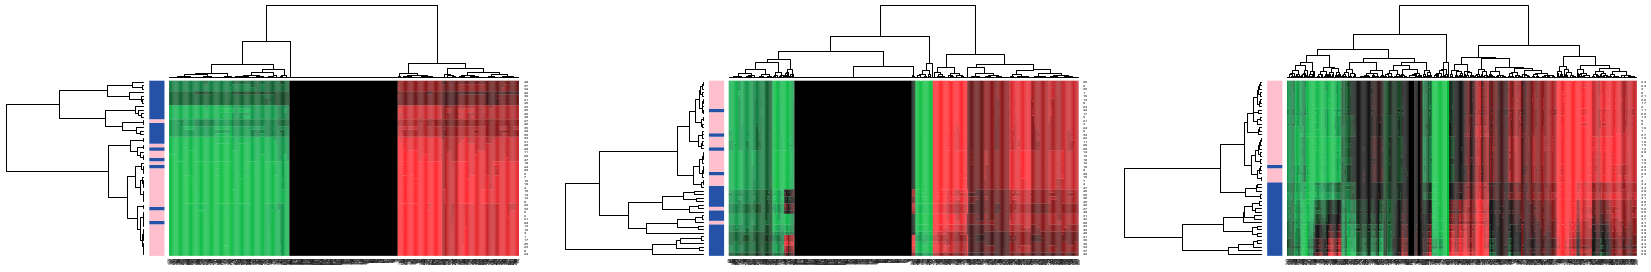
\includegraphics[width=\linewidth]{figures/fig2.png}
    \caption{Mean approximation of colon cancer and the normal matched samples.
      From left to right the methods are HSSVD, FIT-SSVD, and LSHM\@. Colon
      cancer samples are labeled in blue, and normal matched samples are labeled
      in pink in the sidebar.}
  \end{figure}
\end{frame}

\begin{frame}{Hypervariation of Methylation in Cancer (II)}
  \begin{figure}
    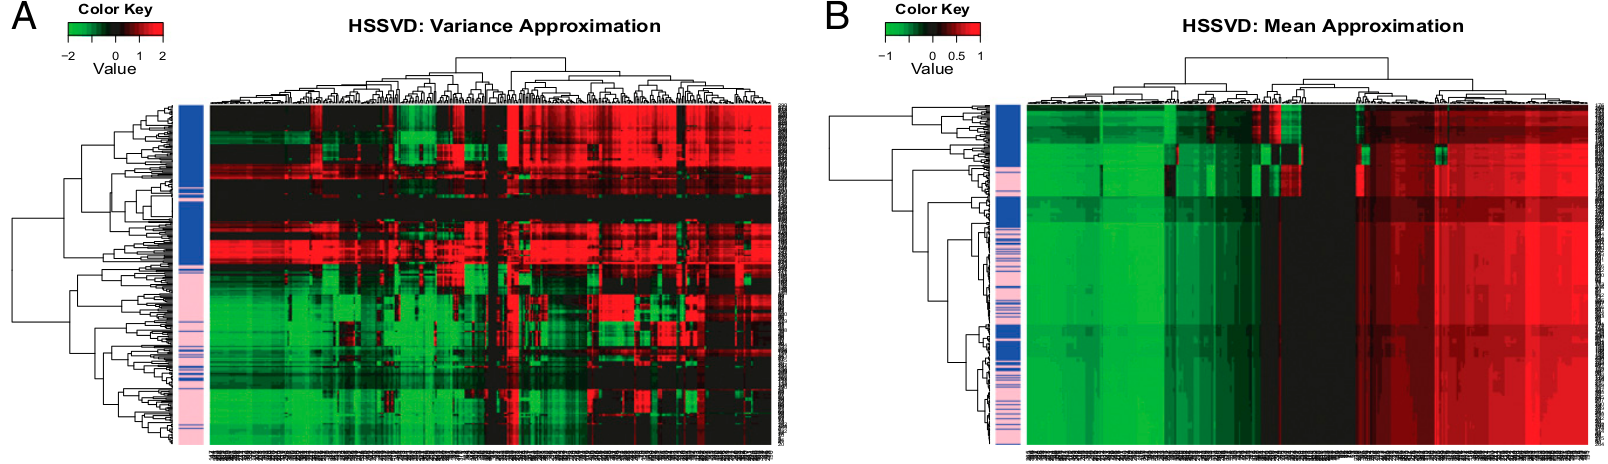
\includegraphics[width=\linewidth]{figures/fig3.png}
    \caption{HSSVD approximation result for all samples. (A) Variance
      approximation; (B) mean approximation. Blue represents cancer samples,
      and pink rep- resents normal samples in the sidebar. Genes and samples
      are ordered by hierarchical clustering. Red represents large values, and
      green represents small values. Only the variance approximation can
      discriminate between cancer and normal samples. More importantly, within
      the same gene, the heatmap for the variance approximation indicates that
      cancer patients have larger variance than normal individuals. This result
      matches the conclusion in ref. 19. In addition, the cDMRs with the
      greatest contrast variance across cancer and normal samples are
      highlighted by the variance approximation, whereas the original paper
      does not provide such information.}
  \end{figure}
\end{frame}

\begin{frame}{Gene Expression in Lung Cancer}
  \begin{figure}
    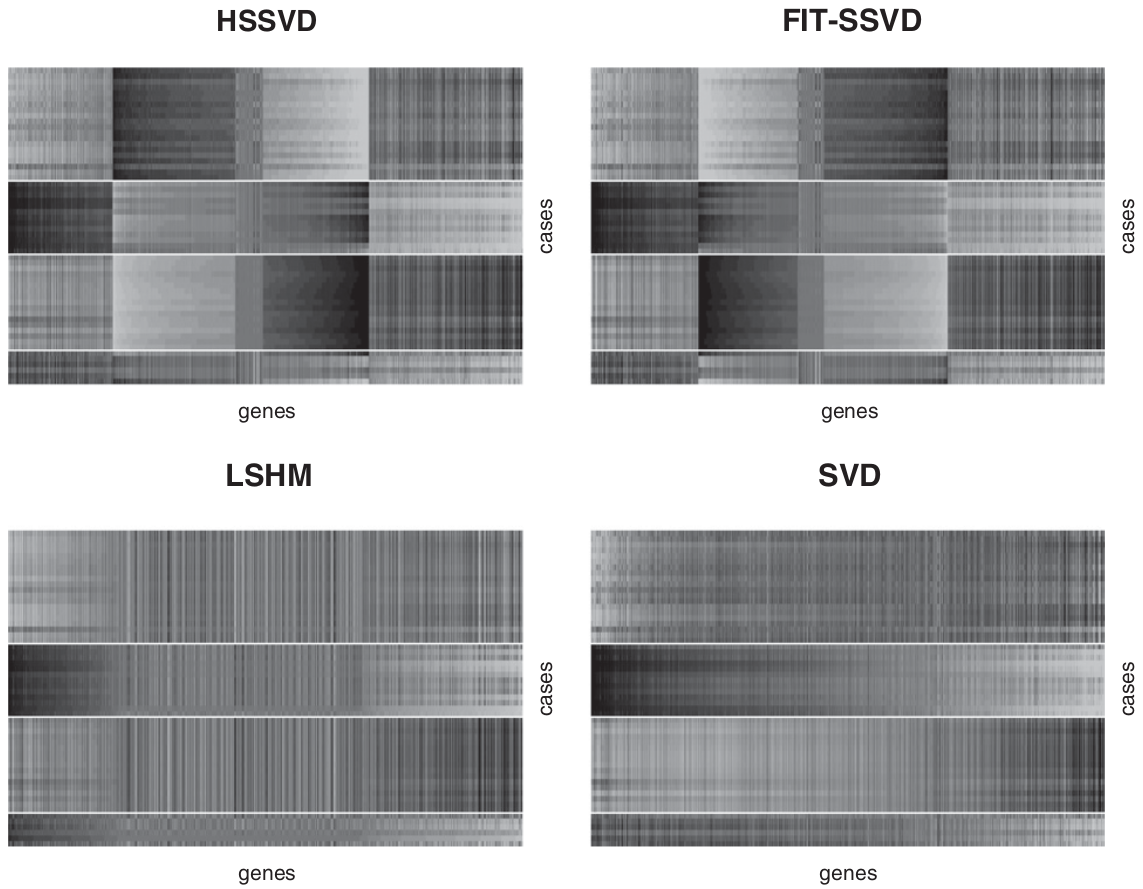
\includegraphics[height=.6\textheight,keepaspectratio]{figures/fig4.png}
    \caption{Checkerboard plots for four methods. We plot the rank-three
      approximation for each method. Within each image, samples are laid in
      rows, and genes are in columns. We order the samples by subtype for all
      images (top to bottom: carcinoid, colon, normal, and small cell), and
      different subtypes are separated by white lines. Genes are sorted by the
      estimated second right singular vector ($\hat{u}_2$), and we only
      included genes that are in the support (defined in Table 1). Across all
      methods, the HSSVD and FIT-SSVD methods provide the clearest block
      structure reflecting biclusters.}
  \end{figure}
\end{frame}

\begin{frame}{Simulated Data}
  \begin{figure}
  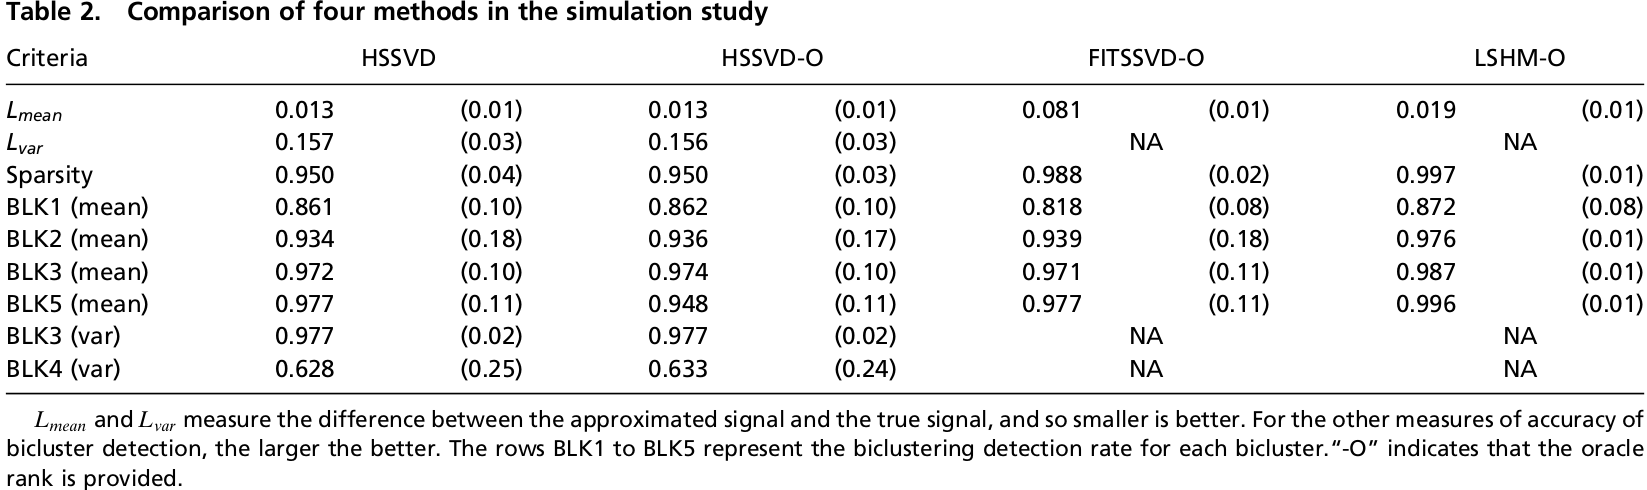
\includegraphics[width=\linewidth,keepaspectratio]{figures/table2.png}
  \end{figure}
\end{frame}

\begin{frame}[label=end, standout]
\end{frame}

\begin{frame}{References}
  \begin{enumerate}
    \item Chen, G., Sullivan, P. F. \& Kosorok, M. R. Biclustering with
      heterogeneous variance. Proceedings of the National Academy of Sciences
      110, 12253–12258 (2013).
    \item Lee, M., Shen, H., Huang, J. Z. \& Marron, J. S. Biclustering via
      Sparse Singular Value Decomposition. Biometrics 66, 1087–1095 (2010).
  \end{enumerate}
\end{frame}

\end{document}
